\renewcommand{\thechapter}{\Roman{chapter}}
\chapter{Methodology}
\renewcommand{\thechapter}{\arabic{chapter}}
\label{ch:Methodology}
\thispagestyle{empty}

In this chapter, the researcher will discuss the materials, methods, and flow that will be using and implementing in the study. First, the researcher will discuss the 3D point cloud scanner. Second, the pre-processing and filtering method of point cloud data will be discussed along with the volume estimation method. Lastly, different testing and evaluation of the study will be addressed. Figure \ref{fig:General flowchart of the system} shows general flowchart of the system. 

\section{3D Point Cloud Scanner}
\label{methdo:sec:System Hardware}

The researcher will adopt the concept of tilting method using a 2D of-the-shelf LiDAR to acquire 3D point cloud data to minimize the cost compared to commercial 3D LiDAR. The hardware and physical components of 3D point cloud scanner are composed of three major components, the 2D LiDAR device, the tilting mechanism which include the fabricated holder for mechanical tilting and the motor for the rotation movement. In Figure \ref{fig:System Hardware Block Diagram}, the 3D point cloud scanner is placed at the top of the flour bin.

\begin{figure}
    \centering
    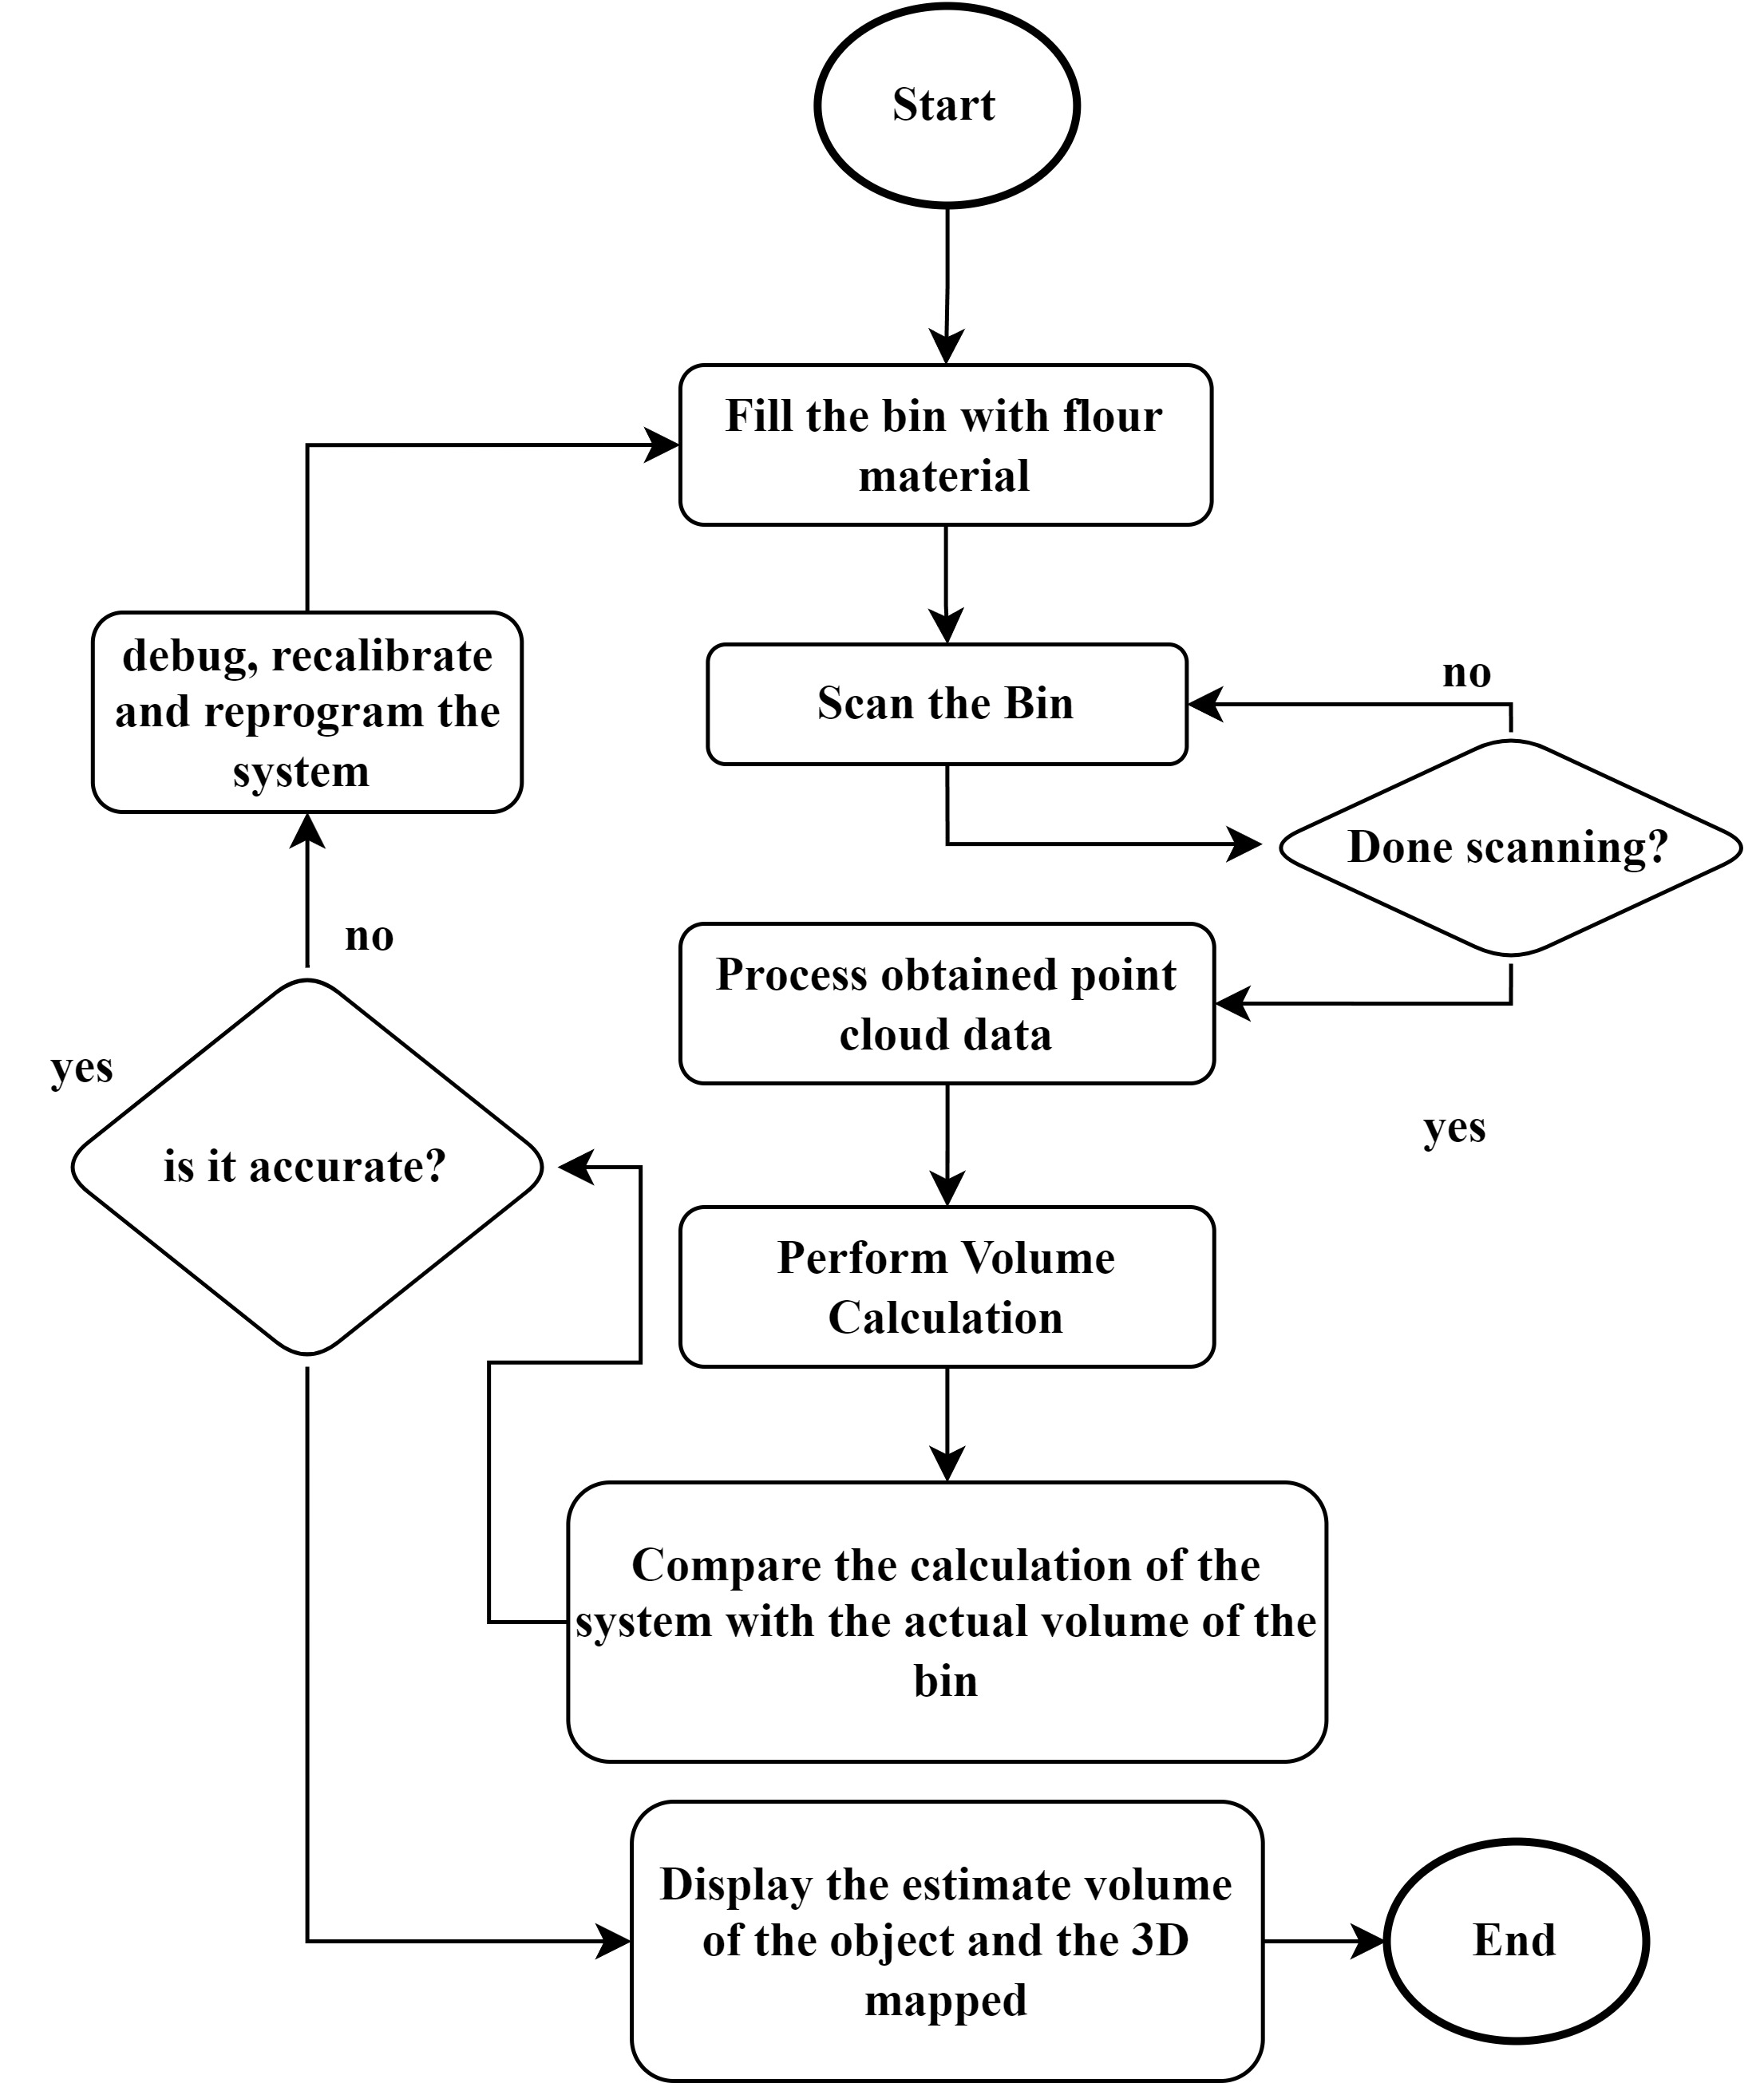
\includegraphics[width=0.9\textwidth]{Figures/general-flowchart-of-the-system-2.jpg}
    \caption{General Flowchart of the System}
    \label{fig:General flowchart of the system}
\end{figure}

\subsection{Modeling of Flour Bin}
\label{method:subsec:Modeling of Flour Bin}
The researcher will model and create a different shapes of the flour bin (e.g. Cylinder, Cube). These different shapes of flour bin will be small-scale and large-scale sizes for testing purposes of the system.

\subsection{Generating of Dust}
\label{method:subsec:Generating of Dust}
The study involves scanning of the bin with the presence of dust, therefore, the researcher will consider to use a blower or fan for generating dust cloud inside the empty space of the bin and flour will be utilize due to its fine-texture. 

\subsection{Data Gathering}
For the data gathering of the raw point cloud, all the major hardware of the system will be assemble and integrate as shown in Figure \ref{fig:System Hardware Block Diagram}. The scanned data from the 2D LiDAR sensor will be received by small computer which is Raspberry Pi for the processing of the raw data. This small computer is connected to the internet in order to control remotely by the personal laptop. Different scanning procedure will be performed to gather point cloud data.

\begin{figure}[H]
    \centering
    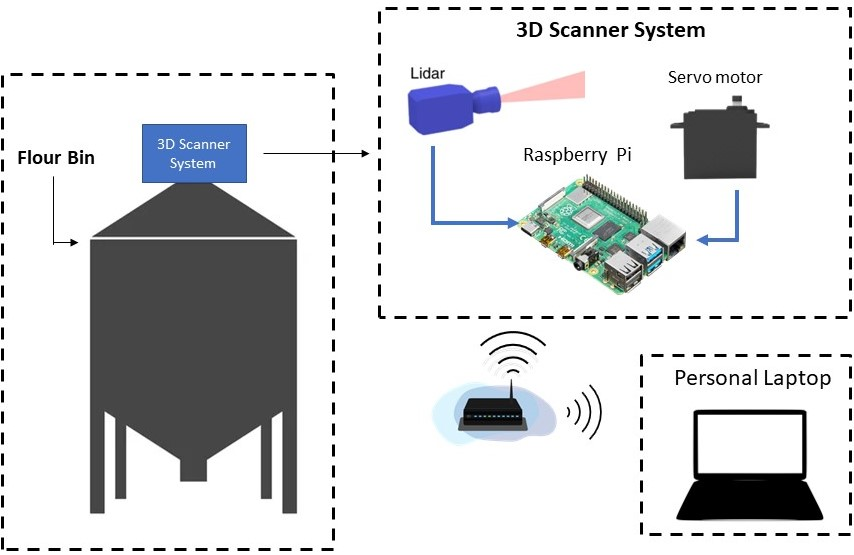
\includegraphics[width=0.9\textwidth]{Figures/system-hardware-block-diagram.jpg}
    \caption{System Hardware Block Diagram}
    \label{fig:System Hardware Block Diagram}
\end{figure}

\section{3D Point Cloud Processing}
\label{method:sec:3D Point Cloud Processing}
The Raspberry Pi will receive the scanned raw data coming from the 3D point cloud scanner. This data will be processed in different stages to produced desired output, such as point cloud pre-processing (formatting, converting, clustering, and cleansing) and post-processing (e.g., 3D mapping and volume measurement). Various platforms and frameworks nowadays are available to ease the handling of these massive raw data, thus, formatting the data to a desired platform must be perform. Typically, the value of raw data coming from the LiDAR sensor is not directly a point cloud data but rather a value of the distance between the sensor and the reflected nearest object in a particular direction, therefore, the data is converted into point cloud which composed of x, y, and z values. The Equation \eqref{eq:x-point}, \eqref{eq:y-point}, and \eqref{eq:z-point} is conversion of polar coordinates (distance, angle) to cartesian coordinates x, y, and z, respectively, in a 3D coordinate system.

\begin{equation}
    x_{point_{i}} = \ \sin(i) \times d \
    \label{eq:x-point}
\end{equation}
\begin{equation}
    y_{point_{i}} = \ \cos(\pi) \times \cos(i) \times d \
    \label{eq:y-point}
\end{equation}
\begin{equation}
    z_{point_{i}} = \ -\cos(i) \times \sin(\pi) \times d \
    \label{eq:z-point}
\end{equation}

Where:

\indent \indent i = scan angle of the scanner

\indent \indent d = the distance point of the emitted pulse by the LiDAR (meter)

\subsection{Point Cloud Data Pre-processing}
The researcher will create an algorithm for clustering and cleansing of the raw data. The data will be clustered into two parts, the outliers (dust) data and the inliers (target) data. Based on the behaviors and characteristics of dust, the researcher will use the Multi-echo method for outlier clustering because the laser emitted by the LiDAR will penetrate through the dust cloud and will receive multiple return. Another method that the researcher will utilize is the low-intensity method clustering for outliers due to the characteristic of the dust having a lower intensity compared to other objects. The data cleansing will be employed after all the data is being clustered. After of these processes, the researcher will convert the pre-processed point cloud for further analysis.

\subsection{Volume Estimation}
\label{method:sec:Volume Estimation}
The researcher will create an algorithm for volume estimation of the material inside the flour bin using Delaunay Triangulation which creates a mesh of triangles such that no point is inside the the circumference of any of the triangle. Convex Hull is a subset of Delaunay Triangulation which creates a boundary on the same given points, all the triangles are on the boundary of the point set. The computation of the estimated volume of the material inside the bin is shown in Figure \ref{fig:volume-estimation-figure} and Equation \eqref{eq:volume-estimation}.

\begin{figure}[H]
    \centering
    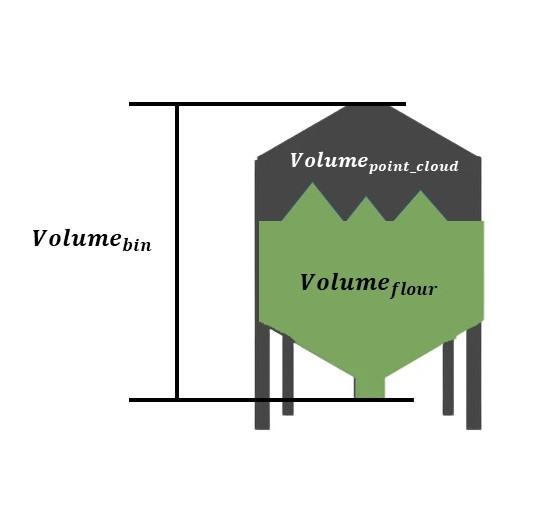
\includegraphics[width=0.8\textwidth]{Figures/volume-estimation-figure}
    \caption{Volume of the flour is the difference between the volume of the bin and volume of the point cloud}
    \label{fig:volume-estimation-figure}
\end{figure}

\begin{equation}
    Volume_{flour} = Volume_{bin} - Volume_{point\_cloud}
    \label{eq:volume-estimation}
\end{equation}

\section{Testing and Evaluation}
\label{method:sec:Testing and Evaluation}
In this section, the researcher will discuss the different testing and evaluation to test and evaluate accuracy of the system.

\subsection{Different Testing Procedure}
\label{method:subsec:Different Testing Procedure}
The researcher will conduct different testing and evaluation to observe the accuracy of the system. In the experiment, the researcher will ensure that the prototype flour bin is scanned remotely and without any human intervention. The researcher intends to perform multiple tests to assess the filtering method and validate the precision and effectiveness of the object's volume measurement, and each of the testing will have a multiple trials. The different testing procedure of the system are the following:
\begin{enumerate}
    \item \label{first} The system will scan the created different shape of flour bin without materials and dust inside.
    \item \label{second} The researcher will generate a dust in the flour bin but without material inside and scan the bin.
    \item \label{third} The searcher will scan the flour bin with flour material inside with different surface shape but without dust.
    \item \label{fourth} The researcher will generate dust from the testing structure conducted in testing \ref{third}
\end{enumerate}

\subsection{Evaluation of the System}
\label{method:subsec:Evaluation of the System}
Based on the conducted different testing mentioned in \ref{method:subsec:Different Testing Procedure}, the researcher will evaluate the conducted testing based on the volume of scanned data. System in the following evaluation

To evaluate the testing \ref{first}, the researcher will measure the accuracy of the system by comparing the estimated volume of the system  with the actual volume of the different shape of the bin, calculate the error percentage for each trial and assess the over all precision of the system. Table \ref{tab:Testing 1} shows the sample comparison of the testing.

\begin{table}[H]
    \caption{Testing \ref{first}}
    \label{tab:Testing 1}
    \centering
    \begin{tabular}{|c|c|c|c|}
        \hline
        % First row
        Flour bin Shape & Actual Volume (\si{mm^3}) & Scanned Volume (\si{mm^3}) & Error (\%) \\
        \hline
        \multicolumn{4}{|c|}{Trial 1} \\
        \hline
        % Second row
        Cube & - & - & - \\
        \hline
        % Third row
        Cylinder & - & - & - \\
        \hline
        \multicolumn{4}{|c|}{Trial 2} \\
        \hline
        Cube & - & - & - \\
        \hline
        % Third row
        Cylinder & - & - & - \\
        \hline
    \end{tabular}
    \end{table}

    Testing \ref{second} will be evaluated from the testing \ref{first} based on the number of point cloud acquired of both testing, and compare it. Basically, the testing \ref{second} will acquired more point cloud compared to testing \ref{first} due to multi-echo or multiple returning from the dust and the flour bin.

In testing \ref{third} and \ref{fourth}, the researcher will place flour materials inside the bin with different surface shape and perform volume estimation. After the volume estimation, the researcher will generate dust, scan the bin, perform volume estimation and compare it to the result of the testing \ref{third}. The sample result of testing \ref{third} and \ref{fourth} is shown in table 

\begin{table}[H]
    \caption{Testing 3 and 4}
    \label{tab:Testing 3 and 4}
    \centering
    \begin{tabular}{|c|p{0.27\linewidth}|p{0.26\linewidth}|p{0.2\linewidth}|}
        \hline
        % First row
        Flour bin Shape & Scanned Volume (without dust) & Scanned Volume (with dust) & Error (\%) \\
        \hline
        \multicolumn{4}{|c|}{Surface Shape 1} \\
        \hline
        % Second row
        Cube & - & - & - \\
        \hline
        % Third row
        Cylinder & - & - & - \\
        \hline
        \multicolumn{4}{|c|}{Surface Shape 2} \\
        \hline
        Cube & - & - & - \\
        \hline
        % Third row
        Cylinder & - & - & - \\
        \hline
    \end{tabular}
    \end{table}